% !Mode:: "TeX:UTF-8" 

\BiChapter{基于注意力机制的神经网络社交媒体文本立场分析}{Methods of inserting figures}

\BiSection{引言}{Figures inserting standard from graduate school}
近年来,有关深度学习的研究越来越深入,在各个领域取得了许多突破。 基于注意力机制的神经网络成为研究的热点,引起了研究者的广泛关注。在神经网络实现预测任务时,注意力机制能使模型更“关注”输入数据中与任务相关的部分,而不是无关部分。在社交媒体文本立场分析任务中,不管是基于传统特征工程的机器学习模型SVM还是基于端到端的深度学习的RNNs,CNNs等神经网络模型,都忽略主题目标信息对社交媒体立场分析的重要作用,这样建立模型存在的不合理性,为提高文本立场分析性能,在本章引入基于注意力机制的神经网络模型。注意力机制能根据主题目标信息对文本信息进行不同重要性的关注,使模型更加聚焦在重要的信息上。实验结果表明,基于注意力机制的神经网络模型在社交媒体文本立场分析任务中取得了相当不错的效果,证明了注意力机制的有效性,同时结合第三章节的条件编码模型,充分利用主题目标信息来挖掘文本立场分析的模式。

本章的各节结构如下:4.2节介绍结合条件编码与注意力机制的神经网络模型的社交媒体文本立场分析;4.3节为本章实验和结果分析;4.4节总结本章的内容。

\BiSection{注意力机制的神经网络模型的社交媒体文本立场分析}{Captions and descriptions of figures}

近年来,基于深度学习的神经网络模型已经在图像识别、语音识别和自然语音处理等领域上取得了重要的进展。在自然语言处理领域中,注意力机制在神经网络机器翻译、序列标注、层次性文档分类上取得突破性提高。

注意力机制将对信息呈现不同的关注程度,通过聚焦在重要的信息上,达到模型性能的特点。将注意力机制应用于文本立场分析任务中。基于不同主题目标对文本信息内容有着不同的侧重点为基础,结合第三章节条件编码技术,本文将文本立场分析中主题目标作为注意力导向,给予文本信息不同权重的关注度,合并授予不同关注度的文本信息中挖掘文本立场分析的模式。


\BiSubsection{注意力机制}{}
注意机制早期应用于图像识别领域。 研究人员的动机也受到人类注意力机制的启发。 在观看图像时,人们并不是一下子看整个图像的每个像素,而是根据需求专注于图像的特定部分。人类将从过去观察到的图像中学习,观察以后应该集中的图像重点。

注意力机制除在图像识别和语音识别上取得巨大的成功,近期在基于RNNs的端到端的编码解码的机器翻译、序列标注和层次文本分类等任务取得突破。在自然语言处理任务中,首先引入注意力机制的是神经网络机器翻译。神经网络机器翻译其实就是一个典型的序列到序列模型,也就是一个编码解码模型。由于基于注意力机制的卷积神经网络模型的注意力机制很类似于机器翻译中的注意力机制,这里将简单介绍下机器翻译中的编码解码注意力机制模型。
\begin{figure}[htbp]
	\centering
	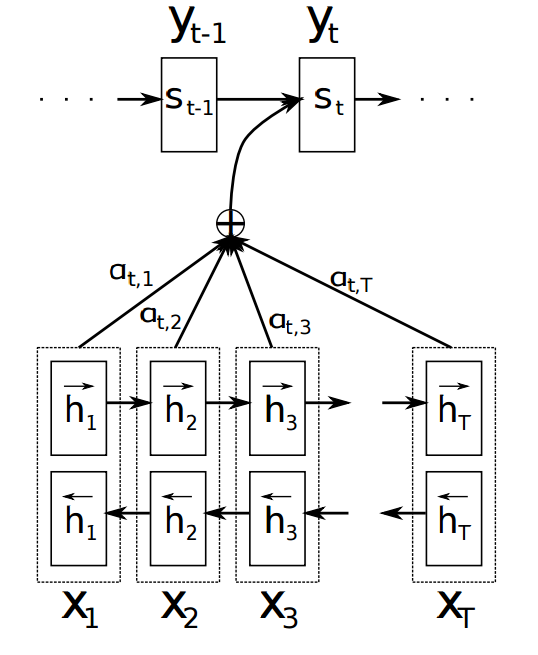
\includegraphics[width = 0.4\textwidth]{NMT.png}
	\caption[rnn_vanish]{注意力机制神经翻译模型}
\end{figure}

传统的神经翻译模型编码阶段里面用的是RNNs模型,这样每个单词的表达不仅能包含前一个单词的信息,还可以包含后一个;RNNs按输入序列的顺序,生成同样顺序的隐藏层状态,这样它就既包含当前单词的前一个单词信息,也包含后一个信息; 这个状态之后将被用于解码阶段部分。
\begin{equation}\label{lstm_f} h_t = f(x_t,h_{t-1}) \end{equation}

其中编码信息为:
\begin{equation}\label{lstm_f} c = q(\lbrace h_1,...h_{T_x} \rbrace ) \end{equation}

其中$h_t$是时间$t$的隐藏状态,$c$向量是从序列信息得到的压缩向量,通常$f$和$q$是非线性函数,例如SutSkever等用的是LSTM作为$f$函数,把前向循环网络的最后一个隐状态当做最后的压缩向量,$q(\lbrace h_1,...h_{Tx} \rbrace )=h_T$。

在解码阶段,解码器的作用是根据编码的信息和已经输出的信息来预测下一个最有可能的单词,可以用公式~\ref{rnndecoder}~表示。
\begin{equation}\label{rnndecoder} p(y) = \prod_{t=1}^{T} p(y_t|\lbrace y1,...,y_{t-1} \rbrace , c) \end{equation}
当$y=(y1,...,y_{T})$,若用RNN式的结构,每个的条件概率如公式\ref{rnndecodery}所示。
\begin{equation}\label{rnndecodery} p(y_t|\lbrace y1,...,y_{t-1} \rbrace , c) = g(y_{t-1},s_t, c)\end{equation}
而基于注意力机制的神经翻译模型的条件概率公式如下。
\begin{equation}\label{} p(y_t|\lbrace y1,...,y_{t-1},x \rbrace,c) = g(y_{t-1},s_t,c_i)\end{equation}
其中$s_i$是RNN的隐状态,其中计算如公式所示。
\begin{equation}\label{} s_i = f(s_{i-1},y_{i-1}, c_i)\end{equation}
其中从传统的神经翻译模型做出的改进是对于每一个不同的输出,它所依据的上下文压缩向量$c_i$不再是同一个压缩向量$c$,$c_i$的计算是通过$(h_1,...,h_{T_x})$的加权所得。$h_i$虽然包含所以所有的输入信息,但是主要存储了$x_i$的信息。其中$c_i$的计算公式如\ref{c1}所示。
\begin{equation}\label{c1} c_i = \sum_{j=1}^{T_x} \alpha_{ij}h_i\end{equation}
其中注意力变量$\alpha_{ij}$的计算如公式所示。
\begin{equation}\label{alpha} \alpha_{ij} = \frac{exp(e_{ij})}{\sum_{k=1}^{T_x}exp(e_{ik})}\end{equation}
其中$e_{ij}$的计算如公式所示。
\begin{equation}\label{eij} \alpha_{ij} = a(s_{i-1},h_j)\end{equation}

注意力机制的加入使得神经网络翻译模型具有更强的对句子翻译建模能力,使模型在翻译当前词语时关注和词语更相关的内容,忽略不相关的内容。通过可视化注意力$\alpha_{ij}$可显示在翻译不同词语时,对原语言关注的内容是不一样的,例如在中文翻译中的注意力矩阵如下图\ref{english2china}所示。
\begin{figure}[htbp]
	\centering
	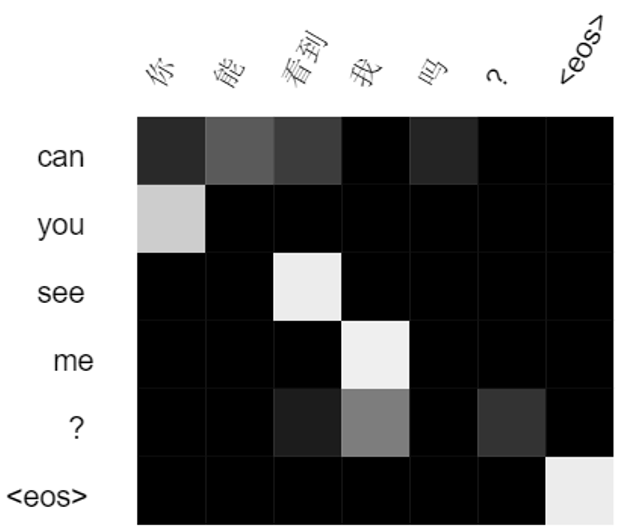
\includegraphics[width = 0.5\textwidth]{mnt_visual.jpg}
	\caption[english2china1]{中英文翻译注意力矩阵}
	\label{english2china}
\end{figure}

\BiSubsection{注意力机制的神经网络模型的社交媒体文本立场分析}{}
基于注意力机制在神经网络翻译模型、序列标注、层次文本分类等领域取得的成功。在社交媒体的文本立场分析上,由于当前研究没有一种有效把主题目标信息以合适的方式结合在文本的立场分析中,但是主题目标对文本立场分析又有着举足轻重的影响。为了弥补主题目标信息没有合适引入的缺点,本文提出一种以注意力机制引入主题目标信息。基于不同主题目标对文本信息内容有着不同的侧重点为基础,结合第三章节条件编码技术,本文将文本立场分析中主题目标作为注意力导向,给予文本信息不同权重的关注度,合并授予不同关注度的文本信息中挖掘文本立场分析的模式。


本节以“深圳禁摩限电”为话题目标,微博文本“支持深圳交警,电单车继续治理”为例,按本节模型的5个层次,描述注意力机制卷积神经网络的立场分析的过程,具体模型的结构如图~\ref{GRU_CNN}~所示。

\begin{figure}[htbp]
	\centering
	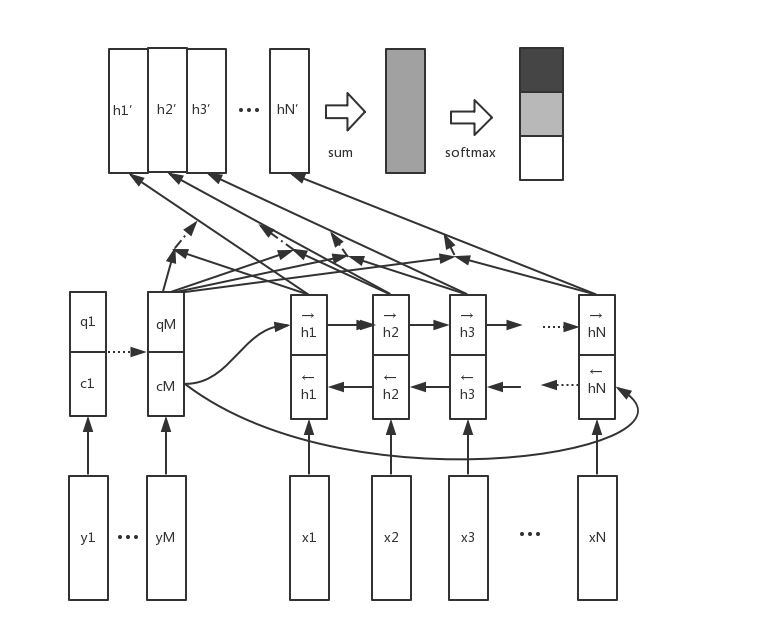
\includegraphics[width = 0.8\textwidth]{a_bi_gru_cnn.png}
	\caption[]{基于注意力机制的神经网络}
	\label{GRU_CNN}
\end{figure}

(1) 输入层

先将话题目标和微博文本经过预处理操作,然后通过分词工具把话题目标和微博文本进行划分,对于同一个话题目标,微博文本分词后句子长度有可能不一致,为了方便后续神经网络框架中的批量的并行计算,英文语料统计选择30为固定长度,中文语料统计后截取50为固定长度,长度超过固定长度进行截断操作,不够的进行补齐词表中规定 <PAD> 关键词。如上述微博文本最后转换成“支持深圳交警。电单车继续治理 <PAD> ... <PAD>”,而话题目标也需要进行分词操作,例如例子中“深圳禁摩限电”根据结巴分词分割成“深圳”、“禁摩”和“限电”三个词组。经过此层后主题目标信息和微博文本信息可以转换成以下形式,$m,n$分别为主题目标和微博文本的长度。
\begin{equation}\label{target_info} Target= \lbrace w_1,w_2...w_m\rbrace \end{equation}
\begin{equation}\label{text_info} Text=\lbrace w'_1,w'_2...w'_n\rbrace  \end{equation}

(2)词向量嵌入层

词向量的嵌入层,此层的功能是对输入的每一次词检索其词向量 (lookup操作),后续实验词向量的预训练由GloVe模型在大量无监督语料上训练得到,预训练的词向量维度为200,且把词向量设置为可训练,随神经网络模型的训练动态调整权重。经过此层后主题目标信息和微博文本信息可以转换成以下形式。
\begin{equation}\label{target_info} Target_v= \lbrace y_1,y_2...y_m\rbrace \end{equation}
\begin{equation}\label{text_info} Text_v=\lbrace x_1,x_2...x_n\rbrace \end{equation}

(3)主题目标编码与文本编码层

由于微博和Twitter文本立场分析中的主题目标包含的词语相对较少,为了减少模型的参数空间,因此编码主题目标信息的方法是单向LSTM模型。微博或Twitter文本包含了文本立场分析的绝大部分信息,双向的LSTM单元能比单向更好抽取文本中的信息,此处采用第三章节提出的条件编码技术编码文本信息,对于当前词的隐藏状态包含前向和后向的LSTM隐状态。具体的转换如以下公式所示。


\begin{equation}\label{lstm_f}[q_1~c_1] = LSTM^{target}(y_1,q_0,c_0)\end{equation}
$$...$$
\begin{equation}\label{lstm_f}[q_m~c_m] = LSTM^{target}(y_m,q_{M-1},c_{m-1})\end{equation}

\begin{equation}\label{lstm_f}[h^{→}_{1}~c^{→}_{1}] = LSTM^{→}(x_1,h_0,c_T)\end{equation}
$$...$$
\begin{equation}\label{lstm_f}[h^{→}_{n}~c^{→}_{n}] = LSTM^{→}(x_n,h^{→}_{n-1},c^{→}_{n-1})\end{equation}

\begin{equation}\label{lstm_f}[h^{←}_{n}~c^{←}_{n}] = LSTM^{←}(x_n,h_0,c_T)\end{equation}
$$...$$
\begin{equation}\label{lstm_f}[h^{←}_{1}~c^{←}_{1}] = LSTM^{←}(x_1,h^{←}_{2},c^{←}_{2})\end{equation}

\begin{equation}\label{lstm_f}h_i= [h^{→}_i~h^{←}_i]\end{equation}

(4)注意力机制计算与基于注意力的隐藏状态合成

通过结合主题目标编码信息$q_m$和微博的文本信息的基于双向LSTM模型的隐状态$h_i$,分别计算主题目标对每个词的关注程度,对于文本分析影响大的词,注意力机制会给予大的权重,反过来对于无用信息,注意力机制则会给予小的权重。分别计算每个词的权重后,原隐状态点乘注意力的权重形成基于注意力的隐藏状态,合并授予不同注意力的隐状态,具体的计算公式如下。
\begin{equation}\label{conv1} e_i=att(h_i,q)=W^t_n(tanh(W_{ah}h_i+W_{aq}q_m+b_a))+b_m \end{equation}
\begin{equation}\label{conv1} a_i=\frac{exp(e_i)}{\sum_{N}^{n=1}exp(e_n)} \end{equation}
\begin{equation}\label{conv1} h'_i=a_i \odot h_i \end{equation}
\begin{equation}\label{conv1} h = h'_i \end{equation}

(5)全连接分类层
把合并授予不同注意力的隐状态当做最后的特征向量,全连接层为Softmax归一化函数,输出的值为归一化到0-1之间的实数值,代表的意义为模型分类到某一个立场的概率,具体公式如下。
\begin{equation}\label{conv1} ouput_i=Softmax(Wh+b) \end{equation}



\BiSection{实验设置及结果分析}{hello}

本节主要介绍基于注意力机制的网络模在NLPCC2016中文微博数据集和SemEval2016英文Twitter数据集中的实验设置及结果分析。通过对样例的可视化注意力机制分析模型是否能抓取对主题目标其关键性作用的信息,解释模型能提高文本立场分析的性能的原因。本节包含两部分: 4.4.1小节简介有关实验的数据集、评价方法、数据预处理词和词向量的训练。4.4.2 小结介绍模型在两个数据集上的结果、对样例的注意力机制可视化结果分析和对比其他模型的结果与分析。


\BiSubsection{实验设置}{}

本章通过在中英文社交媒体数据集上的实验,验证基于注意力机制的神经网络模型在文本立场分析任务上的有效性。数据集包含NLPCC2016中文微博立场分析数据集和SemEval2016英文Twitter立场分析数据集。由于本章实验使用与第三章实验一样的数据集,这里将不再赘述数据集的相关分布,有关数据集的详细分布参考第三章实验章节有关数据集的介绍,训练集、验证集与测试集的划分也与第三章相同。

有关评价方法也与第三章相同,对于同一个数据集内所以主题目标,分别计算其“支持”立场和“反对”立场的F1值,取其两者的平均值作为每个主题的平均F1值。模型在一个数据集上的总体性能通过无差别对待每一个主题目标计算总的“支持”立场与“反对”立场的F1值,两者F1值的平均数作为整个数据集的微平均F1值,微平均F1值代表了模型在数据集上的总体性能,其作为模型最重要的评价指标。有关F1值与微平均F1值的具体计算公式参考第三章的相关介绍。

中英文本数据的预处理步骤主要步骤有转换大小写、过滤停用词与对低频词用“UNKONW”关键词替代。中文本分词工具为结巴分词,英文Twitter的分词为CMU专门为Twitter文本定制的Twitter NLP tool中的分词器。对于英文固定的文本长度为30个词,中文微博为固定60个词。

英文语料的词向量训练通过GloVe算法在20亿Twitter文本语料训练而成,其中包含了120万个词,词向量维度为100。中文微博语料是通过Word2Vec算法在大量微博语料中训练所得,其中包含了17万个词,词向量的维度也为200。


\BiSubsection{实验结果及分析}{}
本文针对中英文数据集内容相差较大的特点,给两个不同的数据集设置不同的超参数,使模型在两个数据集上均取得较好的性能。取出训练集合的10\%作为验证集参与模型的选择。本章提出的基于注意力机制的神经网络的核心超参数主要集中在通过双向LSTM模块进行注意力矩阵和隐藏层的产生的循环神经网络的模块,最后在注意力矩阵作用下的隐藏层提取特征的网络模块。处理英文数据的双向LSTM的隐藏层的单元数为64,处理中文数据的双向LSTM的隐藏层单元数为100。对词向量抽取层的dropout概率为0.2,对LSTM内部记忆单元的dropout概率为0.3,批处理单元样本个数为16。对训练参数的L2正则项为1e-6。选取0.001的学习率的Adam优化方法。模型训练100轮,保留在验证集合性能最好的模型参数。

\begin{table}[htbp]
	\caption[param]{基于注意力机制的神经网络模型超参数集}
	\label{param}
	\vspace{0.5em}\centering\wuhao
	\begin{tabular}{ccc}
		\toprule[1.5pt]
		序号& 超参数名称 &数值\\
		\midrule[1pt]
		0 &词向量大小& 英文 100, 中文 200\\
		1 &LSTM隐藏层单元& 英文 64,中文 100\\
		4 &Embedding层dropout& 0.2\\
		5 &LSTM内部drought& 0.3\\
		6 &批处理大小& 32\\
		7 &L2 正则化参数 &1e-6\\
		8 &全量迭代次数& 50\\
		9 &梯度优化方法& Adam\\
		10 &学习率& 0.001\\
		\bottomrule[1.5pt]
	\end{tabular}
\end{table}

使用上述超参数训练模型,基于注意力机制的网络模型在SemEval2016数据集上的表现表~\ref{a_bi_gru_cnn_semeval}~所示。
\begin{table}[htbp]
	\caption[table123]{基于注意力机制的网络模型在各个话题试验性能(SemEval数据集)}
	\label{a_bi_gru_cnn_semeval}
	\vspace{0.5em}\centering\wuhao
	\begin{tabular}{cccccccc}
		\toprule[1.5pt]
		主题目标& $P_{favor}$&$R_{favor}$&$F_{favor}$&$P_{against}$&$R_{against}$&$F_{against}$&$F_{average}$ \\
		\midrule[1pt]
	Atheism&0.5172&0.4688&0.4918&0.8693&0.8313&0.8498&0.6708\\
	Climate Change&0.7321&1.0000&0.8454&0.0000&0.0000&0.0000&0.4227\\
	Feminist Movement&0.4231&0.3793&0.4000&0.7661&0.7158&0.7401&0.5701\\
	Hillary Clinton&0.4423&0.5111&0.4742&0.6733&0.7907&0.7273&0.6007\\
	Legal. of Abortion&0.6061&0.4348&0.5063&0.7718&0.6085&0.6805&0.5934\\
	合并统计&0.6078&0.6678&0.6378&0.7630&0.7203&0.7416&0.6897\\
		\bottomrule[1.5pt]
	\end{tabular}
\end{table}

如表~\ref{a_bi_gru_cnn_semeval}~所示,以下分析模型的结果。基于注意力机制的网络模型在所有主题目标下微平均F1值的指标为0.6897,其在所有主题目标“支持”立场的F1值为0.6378,而“反对”立场的总体F1值有0.7416。由于原始数据的分布,模型在“反对”立场的性能还是优于“支持”立场,原英文数据集的分布如表~\ref{englishdata}~所示。模型对各个主题目标的性能有较大的差异,在“Athesim”主题目标下性能能达到0.6708,而在主题目标“Climate Change is a Real Concern”中,由于训练集中“支持”立场是“反对”立场的10多倍,模型还是没有克服这个数据分布的缺陷,没有将任意一个样本分类为“反对”立场。

\begin{table}[htbp]
	\caption[table123]{基于注意力机制的网络模型在各个话题试验性能(NLPCC数据集)}
	\label{chinese_a_bi_gru_cnn_semeval}
	\vspace{0.5em}\centering\wuhao
	\begin{tabular}{cccccccc}
		\toprule[1.5pt]
		主题目标& $P_{favor}$&$R_{favor}$&$F_{favor}$&$P_{against}$&$R_{against}$&$F_{against}$&$F_{average}$ \\
		\midrule[1pt]
		iPhone SE&0.6479&0.6133&0.6301&0.6970&0.4423&0.5412&0.5857\\
		春节放鞭炮&0.7263&0.7841&0.7541&0.7912&0.7660&0.7784&0.7662\\
		俄在叙反恐行动&0.6579&0.5319&0.5882&0.5566&0.6860&0.6146&0.6014\\
		开放二胎政策&0.7961&0.8283&0.8119&0.8765&0.7474&0.8068&0.8093\\
		深圳禁摩限电&0.6353&0.8571&0.7297&0.8667&0.8273&0.8465&0.7881\\
		合并统计&0.7000&0.7184&0.7092&0.7550&0.6933&0.7241&0.7167\\
		\bottomrule[1.5pt]
	\end{tabular}
\end{table}

在NLPCC2016数据集上,各主题目标的性能如表~\ref{chinese_a_bi_gru_cnn_semeval}~所示。基于注意力机制的网络模型在所有主题目标下微平均F1值的指标为0.7167,其在所有主题目标“支持”立场的F1值为0.7092,而“反对”立场的总体F1值有0.7241,“支持”立场与“反对”立场在整体的F1值较为相近,因此模型在此数据集上的微平均F1值也比英文数据集高2.70\%。由于中文数据集在各主题目标下立场类标分布相对较平均,没有出现与英文数据集中“Climate Change is a Real Concern”单个主题目标平均F1值只有0.4的结果,但是模型在各个不同主题目标下的性能还是有较大的差距,模型在“开放二胎政策”的主题目标下平均F1值达到了0.8093,但是在“俄在叙反恐行动”主题目标下的平均F1值只有0.581,体现了不同主题目标下,立场分析难易程度也相差较大。


为验证注意力机制与条件编码在结合主题目标信息与文本信息的作用,论证以注意力机制与条件编码能否提高文本立场分析的性能,设计以下对比实验。

双向LSTM独立编码文本信息模型,以下简称\textbf{BiText}

本文第三章所提出的模型,基于条件编码文本的双向LSTM模型结合主题目标信息与文本信息以下简称\textbf{BiText-on-Target}。

以主题目标信息作为注意力机制的导向,对文本信息进行注意力权重的加权模型,以下简称\textbf{Att-BiText}。

以主题目标信息为条件编码文本信息,主题目标信息作为注意力机制的导向,对条件编码后文本信息进行注意力权重加权模型,模型的细节参考图~\ref{GRU_CNN}以下简称\textbf{Att-BiText-on-Target}。

四个模型建模的具体区别如表~\ref{model_list_attention}所示

\begin{table}[htbp]
	\caption[table123]{模型比较}
	\label{model_list_attention}
	\vspace{0.5em}\centering\wuhao
	\begin{tabular}{cccccccc}
		\toprule[1.5pt]
		主题目标&文本编码方式&是否引入主题目标&引入主题目标方式 \\
		\midrule[1pt]
		BiText&双向LSTM&否&无\\
		BiText-on-Target&双向LSTM&是&条件编码\\
		Att-BiText&双向LSTM&是&注意力机制\\
		Att-BiText-on-Target&双向LSTM&是&条件编码\&注意力机制\\
		\bottomrule[1.5pt]
	\end{tabular}
\end{table}

\begin{figure}[htbp]
	\centering
	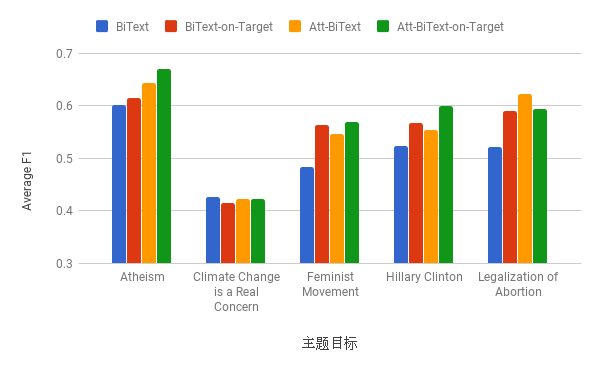
\includegraphics[width = 1.0\textwidth]{chart_attention_condition_semeval.png}
	\caption[rnn_vanish]{对比模型在各主题目标性能分析}
	\label{chart_attention_condition_semeval}
\end{figure}
上述对比模型在英文数据集上各主题目标的平均F1值如图~\ref{chart_attention_condition_semeval}所示,BiText模型除了在“Climate”主题目标上性能能和其他三个模型持平外,在另外4个主题目标下的性能都明显低于引入了主题目标信息的模型,此现象证明了合理引入主题目标信息对文本立场分析有显著的促进作用。第三章所提出的BiText-on-Target模型在“Feminist Movement”与“Hillary Clinton”主题目标下比本章提出的只用注意力机制的神经网络Att-BiText模型性能要高一些,同时Att-BiText模型在“Atheism”和“Abortion”主题目标下性能优于BiText-on-Target模型。因此可以看出两种引入主题目标信息的方式各有优劣,这也促使本文提出融合这两种方式的Att-BiText-on-Target模型。从实验的结果可以看出融合后的Att-BiText-on-Target模型在“Atheism”、“Feminist Movement”与“Hillary Clinton”主题目标下均超过融合前两者的模型,验证了融合条件编码与注意力机制的两种引入主题目标信息的方式的有效性。

汇总各个主题的指标,各模型的总体“支持”与“反对”立场的F1值与微平均F1值如表~\ref{semeval_all_model}~所示。
\begin{table}[htbp]
	\caption[table123]{模型整体性能对比(SemEval数据集)}
	\label{semeval_all_model}
	\vspace{0.5em}\centering\wuhao
	\begin{tabular}{cccccccc}
		\toprule[1.5pt]
		模型& $P_{favor}$&$R_{favor}$&$F_{favor}$&$P_{against}$&$R_{against}$&$F_{against}$&$F_{average}$ \\
		\midrule[1pt]
		BiText&0.5970&0.5263&0.5617&0.7054&0.7902&0.7478&0.6547\\
		BiText-on-Target&0.5743&0.6480&0.6112&0.7396&0.7231&0.7314&0.6713\\
		Att-BiText&0.5778&0.6842&0.6310&0.7707&0.6629&0.7168&0.6739\\
		Att-BiText-on-Target&0.6078&0.6678&0.6378&0.7630&0.7203&0.7416&0.6897\\
		\bottomrule[1.5pt]
	\end{tabular}
\end{table}

\begin{table}[htbp]
	\caption[table123]{模型整体性能对比(NLPCC数据集)}
	\label{semeval_all_model}
	\vspace{0.5em}\centering\wuhao
	\begin{tabular}{cccccccc}
		\toprule[1.5pt]
		模型& $P_{favor}$&$R_{favor}$&$F_{favor}$&$P_{against}$&$R_{against}$&$F_{against}$&$F_{average}$ \\
		\midrule[1pt]
		BiText&0.6565&0.6706&0.6636&0.7186&0.6892&0.7039&0.6837\\
		BiText-on-Target&0.6721&0.6850&0.6785&0.7146&0.7219&0.7182&0.6984\\
		Att-BiText&0.6537&0.7208&0.6872&0.7506&0.6646&0.7076&0.6974\\
		Att-BiText-on-Target&0.7000&0.7184&0.7092&0.7550&0.6933&0.7241&0.7167\\
		\bottomrule[1.5pt]
	\end{tabular}
\end{table}

BiText模型在中英文数据集中取得0.654和0.683的微平均F1值,以条件编码引入主题目标信息的BiText-on-Target模型在中英文数据集上的微平均F1值为0.671与0.698。以条件编码引入主题目标信息显著的提升了模型的性能,第三章也有相应的实验论证了上述结论。以注意力机制引入主题目标信息的Att-BiText模型在在中英文数据集上的微平均F1值为0.671与0.697。与条件编码的模型性能相近,但从在英文数据集上各主题目标的性能分析图~\ref{model_list_attention}中可以看出,两模型在不同的主题目标任务下各有优劣。因此本文提出融合条件编码与注意力机制这两种引入主题目标信息的Att-BiText-on-Target模型。

Att-BiText-on-Target模型在中英文数据集上取得微平均F1值分别为0.689与0.716,相对于BiText模型分别提高了3.5\%与3.3\%,相对于不引入主题目标信息有显著的提升。Att-BiText-on-Target模型相对于单独的条件编码的BiText-on-Target分别提升了1.7\%1.9\%,相对于单独的注意力机制的Att-BiText模型分别提高了1.4\%与1.8\%。表明融合两种引入主题目标信息方法在中英文数据集上都取得高于原模型的性能,从各主题目标任务下性能分析图~\ref{model_list_attention}可知Att-BiText-on-Target模型在“Atheism”、“Feminist Movement”与“Hillary Clinton”主题目标下有着显著的提升。总上所述,对比实验验证融合注意力机制与条件编码两种引入主题目标信息的Att-BiText-on-Target模型的有效性。

为了验证本章提出的融合条件编码与注意力机制的网络模型的有效性和不足之处,以下通过实验结果对比其他研究人员在文本研究中模型。由于两个数据集来源于不同的评测任务,因此分别从SemEval2016英文数据集和NLPCC2016中文数据集挑选出较好系统和本章提出的基于注意力机制的网络模型进行比较。

在SemEval数据集合上,引入以下模型是作为对比模型。

(1)MITRE \citeup{zarrella2016mitre}, SemEval2016 Twitter立场分析评测任务第一名,模型详细介绍参考第三章实验部分。

(2)SVM  \citeup{mohammadstance} 2017 Mohammad所提出基于n-gram,POS,sentiment等特征的SVM模型

(3)BiText-On-Target 第三章提出的基于主题目标的条件的双向LSTM文本编码模型,模型详细介绍参考第三章实验部分。

(4) Att-BiText-on-Target 本章提出的结合注意力机制与条件编码的神经网络模型。

四个模型在SemeEval2016的各主题目标下单个平均F1值如图~\ref{chart_semeval_best_model_attention}~所示。
\begin{figure}[htbp]
	\centering
	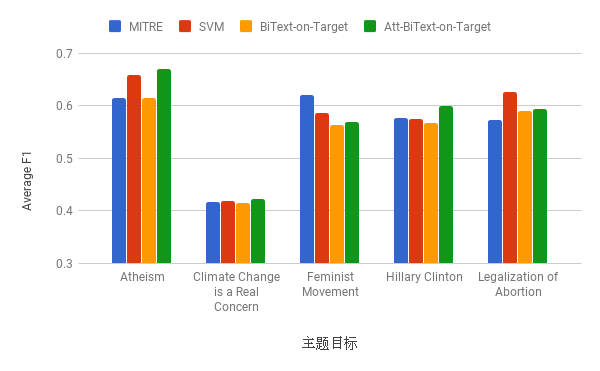
\includegraphics[width = 1.0\textwidth]{chart_semeval_best_model_attention.png}
	\caption[rnn_vanish]{模型在SemeEval2016各主题目标平均F1值分布}
	\label{chart_semeval_best_model_attention}
\end{figure}

本文提出的融合条件编码与注意力机制的网络模型在“Atheism”、”Climate Change is a Real Concern“和“Hillary Clinton”主题目标下分别取得了0.671、0.423和0.600的平均F1值,均在四个模型中取得最佳性能。基于特征工程的模型SVM在“Legal of Abortion”依旧取得最高性能,比其他三个基于深度学习的模型都要高,其具体的原因可能是在此主题目标上分类需要建立人工参与的特征,而深度学习模型在数据较少的情况下无法提取出此类特征。融合条件编码与注意力机制网络模型在英文数据集各个话题中都取得较高的性能,一定程度反应了此模型在解决文本立场分析中的有效性。

上述模型在SemEval数据集下的综合“支持”和“反对”的F1值和总体微平均F1值的性能如下表~\ref{semeval_attention_res}~所示。


本章提出的融合条件编码与注意力机制网络在英文数据集总体的“支持”立场的F1值为0.637,“反对”立场的F1值为0.747,总体立场分析的微平均F1值为0.689。对比其他三个模型,融合条件编码与注意力机制网络在“反对”立场平均F1值与总体微平均F1值均取得最高性能。比只用条件编码的BiText-On-Target模型高1.7\%。Att-BiText-on-Target优于SemEval所有评测模型,微平均F1值比评测任务的最佳模型MITRE高1.08\%,比Mohammad在2017所提出的基于n-gram,POS,sentiment等特征的SVM模型高0.60\%。MITRE模型需要大量的无标注Twitter语料,SVM模型需要手工构造一些人为选择的特征。从上述对比中验证融合条件编码与注意力机制的网络模型在英文Twitter立场分析有效性。

\begin{table}[htbp]
	\caption[table123]{各模型在立场分析测试集中的性能表现(SemEval 数据集)}
	\vspace{0.5em}\centering\wuhao
	\label{semeval_attention_res}
	\begin{tabular}{cccccccc}
		\toprule[1.5pt]
		模型& $F_{favor}$&$F_{against}$&$F_{average}$ \\
		\midrule[1pt]
		MITRE\citeup{zarrella2016mitre}&0.5932&0.7633&0.6782\\
		SVM\citeup{mohammadstance} &-&-&0.6830\\
		BiText-On-Target&0.6112&0.7314&0.6713\\
			Att-BiText-on-Target&0.6378&0.7478&0.6897\\
		\bottomrule[1.5pt]
	\end{tabular}
\end{table}

上述统计说明模型在SemEval英文数据的性能,以下将在NLPCC2016中文数据集对比评测中的模型,对比的模型如下所示。

(1)RUC-MMC\citeup{xu2016overview} NLPCC2016 立场分析评测任务第一名,提模型详细介绍参考第三章实验部分。

(2)Top-Team \citeup{xu2016overview}NLPCC2016立场分析评测任务参赛模型,为模型详细介绍参考第三章实验部分。

(3) BiText-On-Target 第三章提出的基于主题目标的条件的双向LSTM文本编码模型,模型详细介绍参考第三章实验部分。

(4) Att-BiText-on-Target 本章提出的结合注意力机制与条件编码的神经网络模型。

四个模型在SemeEval2016的各主题目标下单个平均F1值如图~\ref{chart_nlpcc_best_model_attention}~所示。
\begin{figure}[htbp]
	\centering
	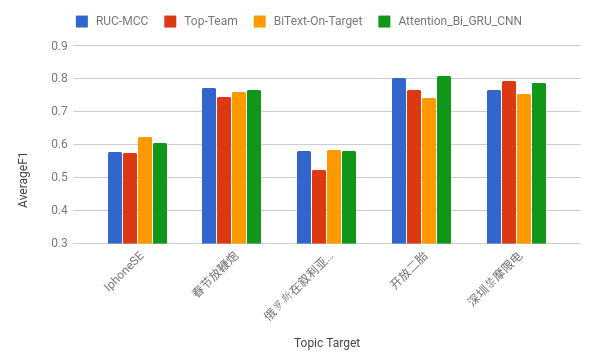
\includegraphics[width = 1.0\textwidth]{chart_nlpcc_best_model_attention.png}
	\caption[rnn_vanish]{模型在NLPCC2016各主题目标平均F1值分布}
	\label{chart_nlpcc_best_model_attention}
\end{figure}


本章节提出融合条件编码与注意力机制网络模型在“开发二胎”主题目标下0.809的平均F1值,并在“深圳禁摩限电”主题目标下取得0.7881的平均F1值的。基于提取主题目标的关键字典的Top-Team在“深圳禁摩限电”主题目标上取得最好的0.794平均F1值,说明基于特征的传统机器学习方法解决特定主题目标还是有一定的优势的。融合条件编码与注意力机制的网络模型在三个“IphoneSE”、“开放二胎”和“深圳禁摩限电”主题目标下平均F1值均高于评测系统最佳RUC-MCC模型。通过融合第三章所提出的条件编码模型,Att-BiText-on-Target模型在“春节鞭炮”,“俄罗斯反恐行动”,“开放二胎”,“深圳禁摩限电”四个主题目标任务下均比原模型条件编码BiText-On-Target具备更好的性能。融合条件编码与注意力机制网络模型在三个主题目标均取得最优性能,并且在其余两个主题目标下也有相对较好的性能,说明模型在中文文本立场分析任务中的有效性。

上述模型在NLPCC数据集下的综合“支持”和“反对”的F1值和总体微平均F1值的性能如下表~\ref{nlpcc_res_attention}~所示。
\begin{table}[htbp]
	\caption[table123]{各模型在立场分析测试集中的性能表现(NLPCC 数据集)}
	\label{nlpcc_res_attention}
	\vspace{0.5em}\centering\wuhao
	\begin{tabular}{cccccccc}
		\toprule[1.5pt]
		模型& $F_{favor}$&$F_{against}$&$F_{average}$ \\
		\midrule[1pt]
		RUC-MMC\citeup{xu2016overview}&0.6969&0.7243&0.7106\\
		Top-Team\citeup{xu2016overview}&0.6601&0.7186&0.6894\\
		BiText-On-Target&0.6761&0.7158&0.6984\\
		A-Bi-GRU-CNN&0.7092&0.7241&0.7167\\
		\bottomrule[1.5pt]
	\end{tabular}
\end{table}

本章节提出融合条件编码与注意力机制网络模型在NLPCC2016数据集上取得“支持”立场平均F1值为0.7092,“反对”立场的平均F1值为0.7241,总体微平均F1值为0.716,在所对比模型中取得最优性能,模型性能比NLPCC最好的模型RUC-MMC在微平均上高了0.61\%,说明模型在中文立场分析任务中的有效性。模型比第三章节提出的基于条码编码的BiText-On-Target模型高了1.7\%。证明在中文文本立场分析中,融合条件编码与注意力机制网络模型比条件编码模型更能建模有主题目标信息和文本信息的立场分析任务。


\BiSection{本章小结}{}

本章介绍了基于注意力机制的网络模型在文本立场分析上的工作。受注意力机制在图像处理、语音识别、机器翻译上性能的突破,将注意力机制应用于文本立场分析任务中。将文本立场分析中主题目标作为注意力导向,给予文本信息不同权重的关注度,其后在已经授予不同关注度文本信息中挖掘有关立场分析的模式。同时受到第三章所提出条件编码能更好的编码文本信息的启发,融合了条件编码与注意力机制这两种引入主题目标信息的方法。为验证最终模型的有效性,分别在中英文数据集上进行了实验,在SemEval2016英文数据集上取得0.689的微平均F1值,相对于评测最优系统提升了1.08\%,相对于Mohammad在2017年提出的基于特征的SVM模型提高了0.60\%。在NLPCC中文数据集上取得0.7167的微平均F1值,相对于评测最优系统提高了0.61\%。本章节提出的融合条件编码与注意力机制网络模型在中英文均取得很好的性能。证明了的融合条件编码与注意力机制网络模型在文本立场分析任务上是有效的。



